\section{Design Front-end}
\label{sec:design}

\textbf{Premessa.} In questa sezione sono illustrate le specifiche visuali, i wireframe e le tavole grafiche del design system ``Strumento Civico'' per l'interfaccia di \textbf{TEPO}. I design board e i mockup di riferimento --- allestiti su Canva a partire dalle linee guida editoriali dello strumento civico --- costituiscono il riferimento visuale della baseline per i requisiti e la matrice di tracciabilità, garantendo la separazione tra la progettazione visuale/UX e le schermate di collaudo che verranno integrate nel D2. Nelle figure seguenti sono illustrate le composizioni di interfaccia nel registro \emph{Relazione} e nel registro \emph{Sala operativa}.

Tutte le schermate adottano lo stesso insieme di regole visive: una fascia di stato con i numeri di sintesi, un indice numerato raggruppato in \emph{Decisione} e \emph{Dati}, filetti da un pixel, titoli editoriali, micro-etichette e cifre tabellari. I due registri di lettura --- \emph{Relazione} (carta) e \emph{Sala operativa} (grafite) --- condividono layout e informazione e cambiano soltanto il materiale cromatico e tipografico. Le immagini non dimostrano da sole il soddisfacimento di requisiti non funzionali come compatibilità o prestazioni: quei requisiti sono verificati con le modalità descritte nella Sezione~\ref{sec:RNF}.

\subsection{Shell, navigazione e Dashboard}
\begin{figure}[H]
    \centering
    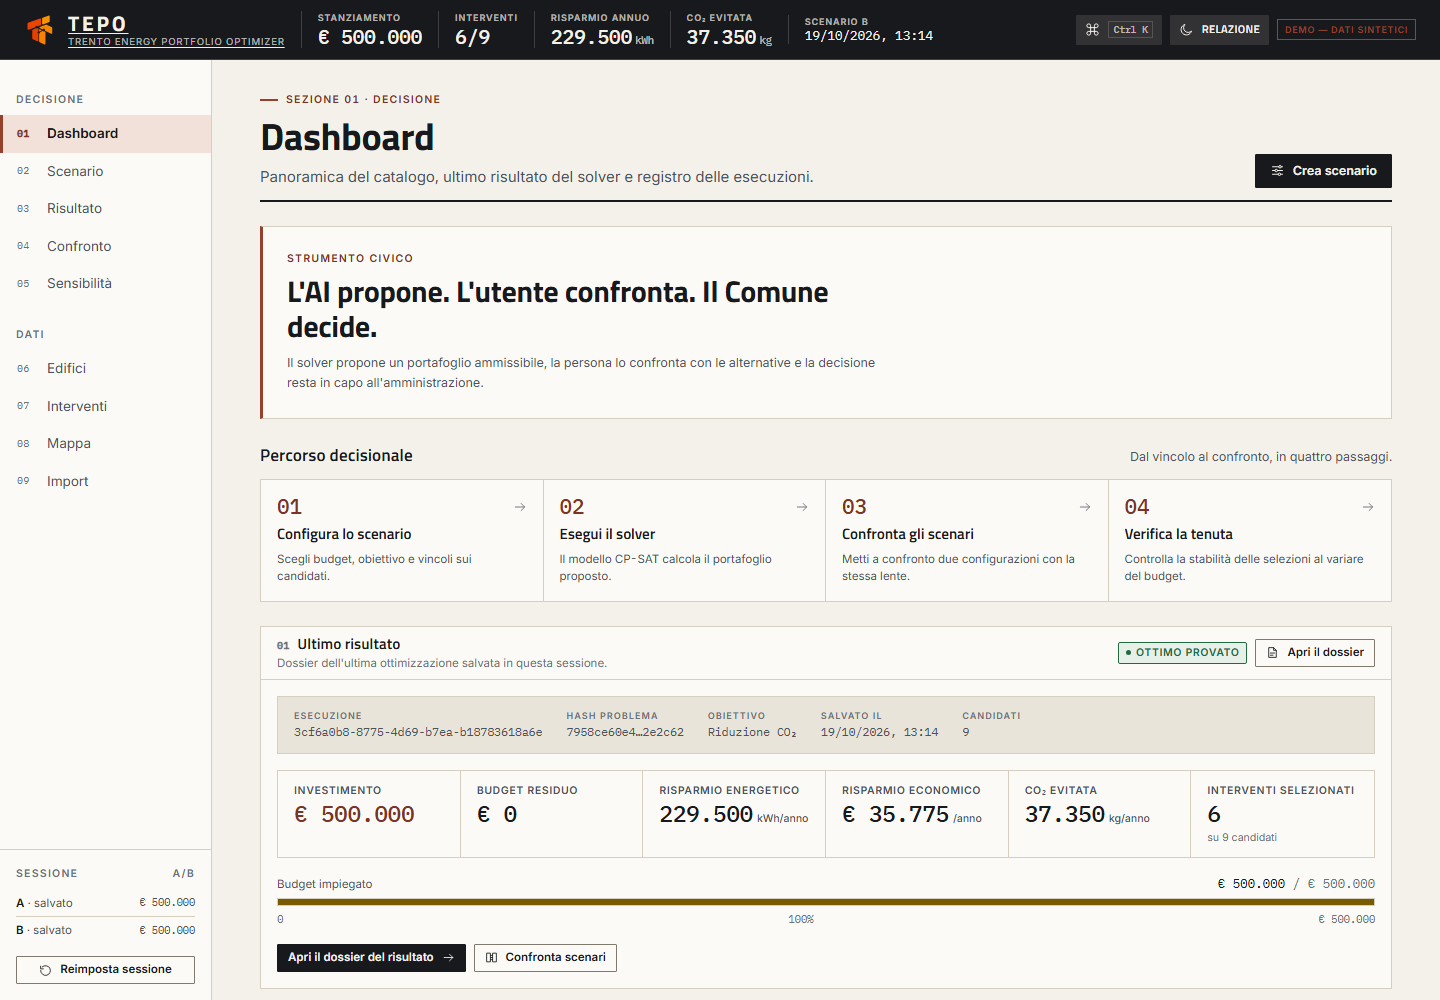
\includegraphics[width=0.95\linewidth]{img/dashboard-relazione.png}
    \caption{MU-Fig.1 --- Shell dell'applicazione e Dashboard nel registro Relazione.}
    \label{fig:shell}
\end{figure}

La Figura~\ref{fig:shell} mostra la shell comune a tutte le pagine e la dashboard iniziale. La \emph{fascia di stato} espone in modo permanente lo stanziamento, il rapporto tra interventi selezionati e candidati, il risparmio annuo, la CO\textsubscript{2} evitata, l'ultimo scenario o risultato, il comando dei comandi rapidi (\texttt{Ctrl/Cmd + K}), il cambio registro e il timbro \textbf{DEMO --- dati sintetici}. L'\emph{indice numerato} a sinistra raggruppa le sezioni in \textbf{Decisione} (Dashboard, Scenario, Risultato, Confronto, Sensibilità) e \textbf{Dati} (Edifici, Interventi, Mappa, Import); in fondo è presente il pannello \textbf{Sessione A/B} con l'occupazione degli slot e il comando ``Reimposta sessione''. La \emph{dashboard} riporta il manifesto dello strumento (``L'AI propone. L'utente confronta. Il Comune decide.''), il percorso decisionale in quattro passi, il dossier dell'ultimo risultato, il registro delle ultime esecuzioni e gli indicatori del catalogo.

Collegamenti principali: \RFref{rf:catalogo_edifici}, \RFref{rf:config_scenario}, \RFref{rf:ottimizzazione}, \RFref{rf:risultati}, \RFref{rf:storico}, \RFref{rf:scenari_salvati}, \RFref{rf:tema}, \RFref{rf:provenienza}; UC-01, UC-05, UC-07, UC-08, UC-09, UC-15; US-01, US-05, US-07, US-08, US-10, US-11, US-16, US-17.

\subsection{Registro Sala operativa}
\begin{figure}[H]
    \centering
    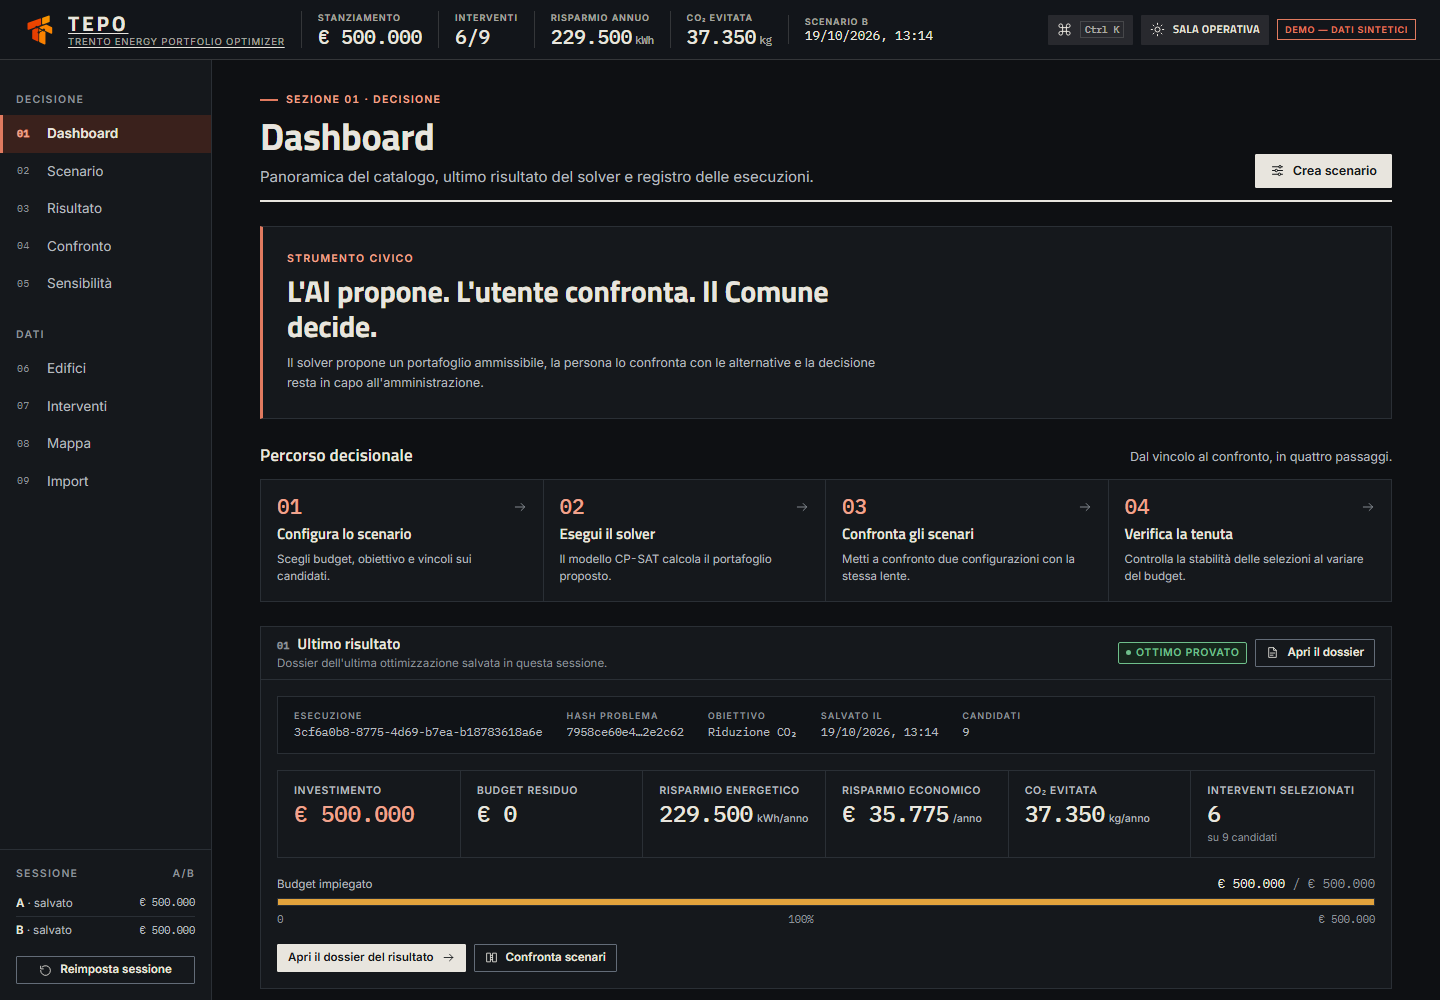
\includegraphics[width=0.95\linewidth]{img/dashboard-sala-operativa.png}
    \caption{MU-Fig.2 --- La stessa dashboard nel registro Sala operativa.}
    \label{fig:sala-operativa}
\end{figure}

La Figura~\ref{fig:sala-operativa} mostra lo stesso contenuto della Figura~\ref{fig:shell} nel registro \emph{Sala operativa}: layout e informazione non cambiano, cambia il materiale cromatico. Il registro può essere cambiato dalla fascia di stato o dalla palette dei comandi rapidi, viene conservato tra le sessioni e alla prima apertura segue la preferenza del sistema operativo. In stampa il sistema impone uno sfondo chiaro con inchiostro scuro ed elimina navigazione e controlli.

Collegamenti principali: \RFref{rf:tema}, \RFref{rf:risultati}; UC-15; US-16.

\subsection{Catalogo degli edifici}
\begin{figure}[H]
    \centering
    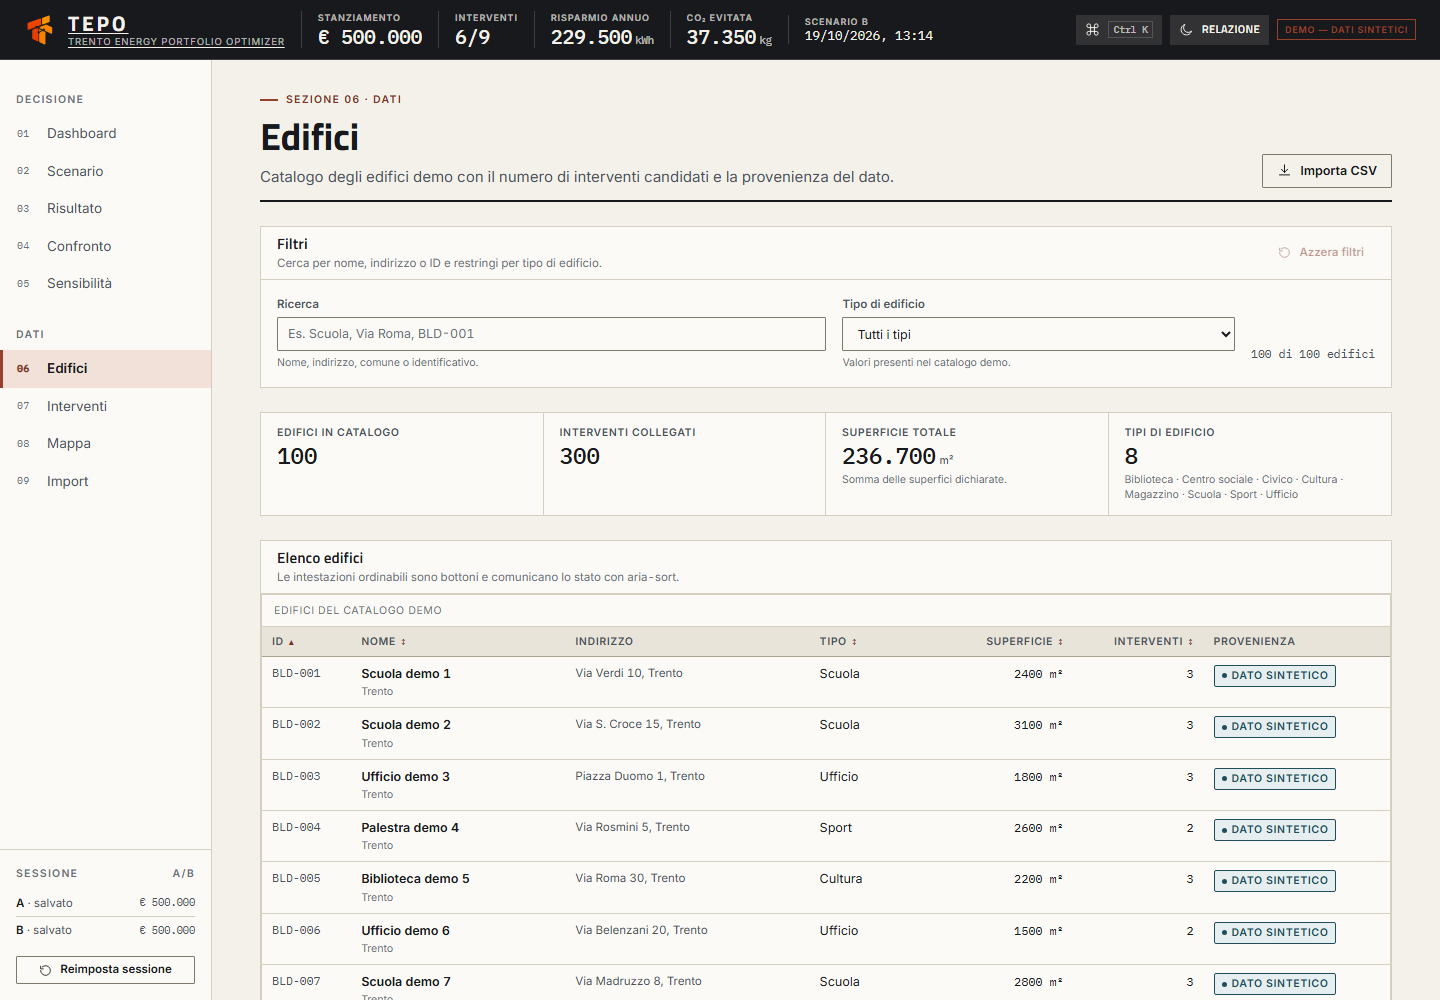
\includegraphics[width=0.95\linewidth]{img/edifici.png}
    \caption{MU-Fig.3 --- Catalogo degli edifici con filtri, indicatori e provenienza del dato.}
    \label{fig:edifici}
\end{figure}

La Figura~\ref{fig:edifici} mostra il catalogo degli edifici. Sono presenti i filtri per ricerca testuale e tipologia, il comando per azzerare i filtri, il contatore degli edifici visualizzati, quattro indicatori sintetici (edifici in catalogo, interventi collegati, superficie totale, tipi di edificio) e la tabella con identificativo, nome e comune, indirizzo, tipologia, superficie, numero di interventi e provenienza del dato. Le intestazioni ordinabili sono pulsanti che comunicano lo stato di ordinamento agli strumenti assistivi; il comando ``Importa CSV'' conduce alla pagina di importazione.

Collegamenti principali: \RFref{rf:catalogo_edifici}, \RFref{rf:provenienza}; UC-01, UC-04; US-01, US-04, US-17.

\subsection{Catalogo degli interventi}
\begin{figure}[H]
    \centering
    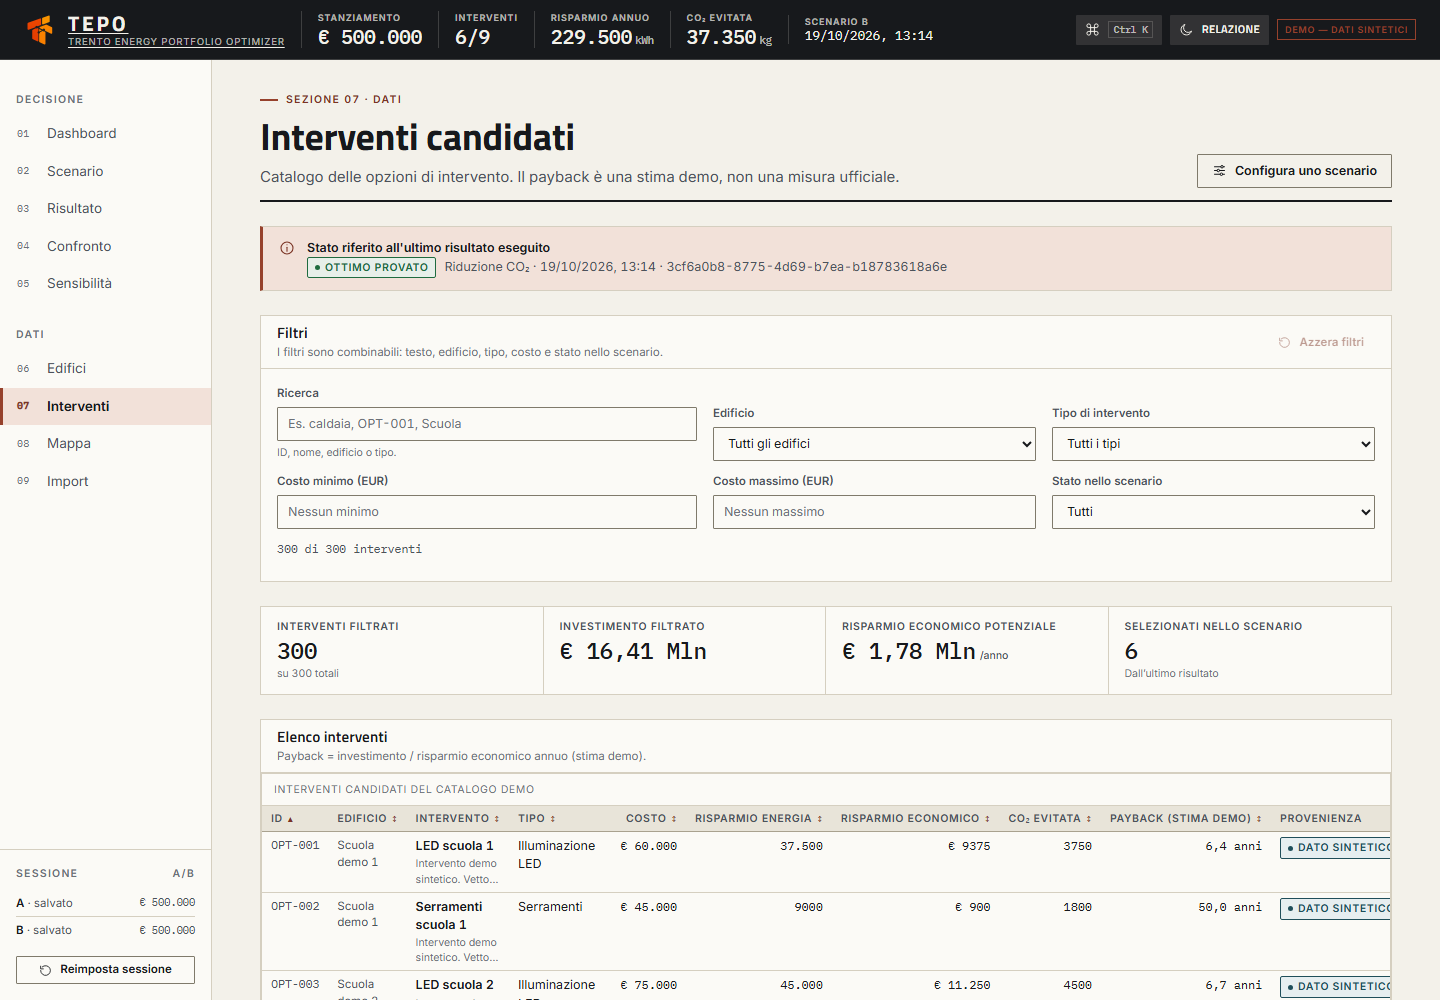
\includegraphics[width=0.95\linewidth]{img/interventi.png}
    \caption{MU-Fig.4 --- Catalogo degli interventi con filtri combinabili e stato nello scenario.}
    \label{fig:interventi}
\end{figure}

La Figura~\ref{fig:interventi} mostra il catalogo degli interventi. La pagina espone un avviso che collega lo stato delle opzioni all'ultimo risultato eseguito (oppure dichiara che nessuno scenario è stato eseguito), i filtri combinabili (ricerca testuale, edificio, tipo di intervento, costo minimo e massimo, stato nello scenario), quattro indicatori del sottoinsieme filtrato e la tabella con identificativo, edificio, intervento, tipologia, costo, risparmio energetico, risparmio economico, CO\textsubscript{2}, payback (stima demo), provenienza e stato. La pagina è collegata alla configurazione dello scenario.

Collegamenti principali: \RFref{rf:catalogo_interventi}, \RFref{rf:filtri_interventi}, \RFref{rf:provenienza}; UC-03, UC-05; US-03, US-17.

\subsection{Scenario Builder}
\begin{figure}[H]
    \centering
    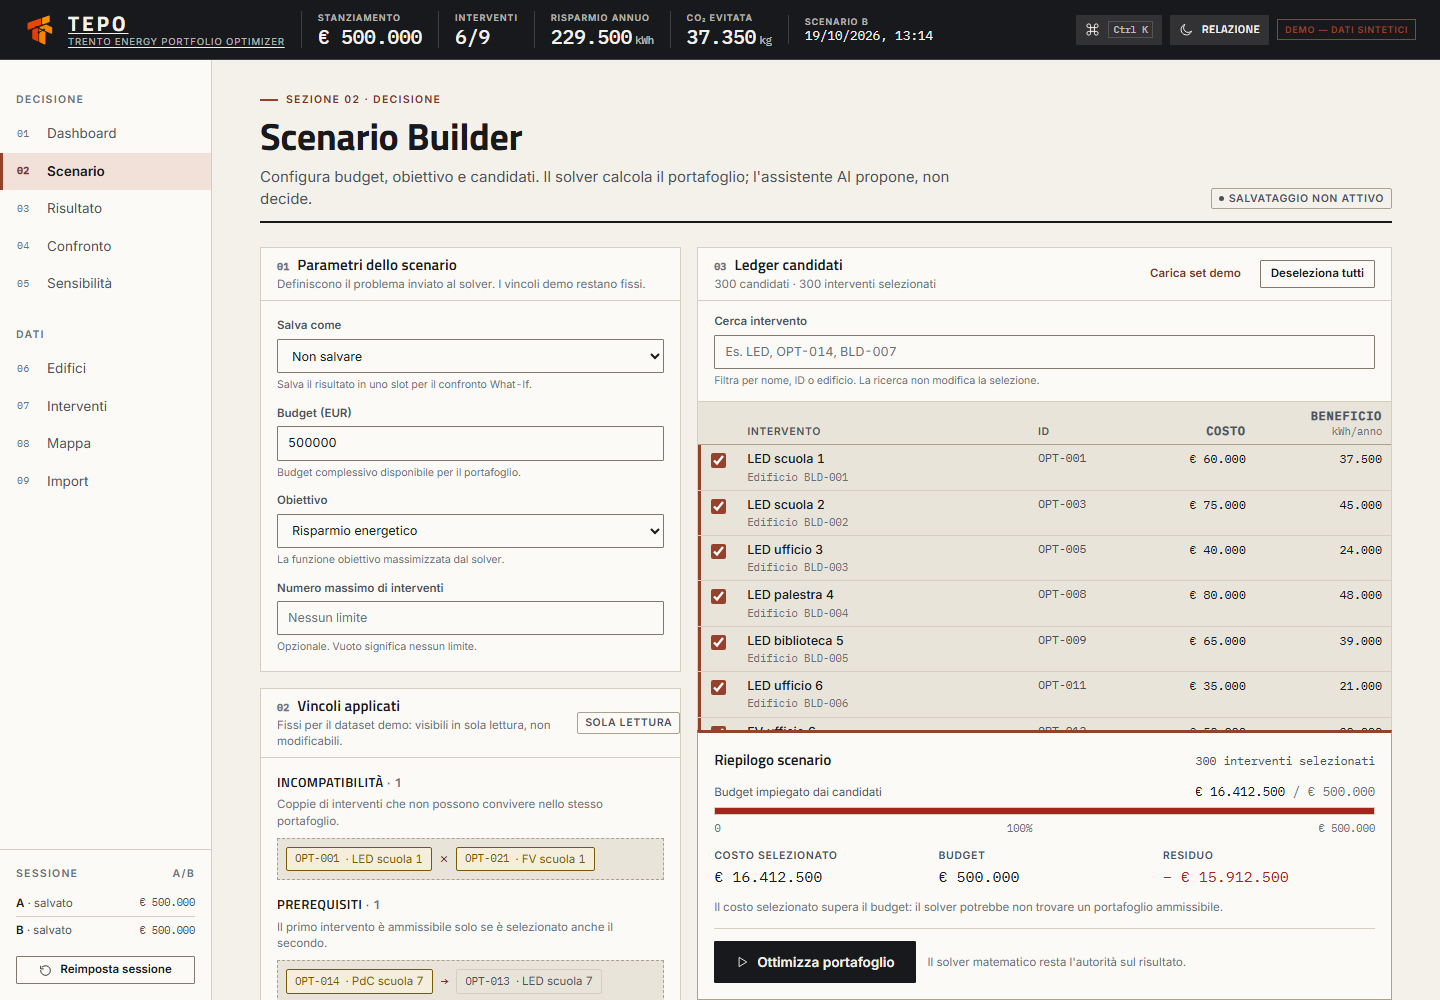
\includegraphics[width=0.95\linewidth]{img/scenario.png}
    \caption{MU-Fig.5 --- Scenario Builder: parametri, vincoli, ledger dei candidati e riepilogo.}
    \label{fig:scenario}
\end{figure}

La Figura~\ref{fig:scenario} mostra lo \emph{Scenario Builder}, articolato in due colonne. A sinistra sono presenti i parametri dello scenario (scelta dello slot di salvataggio, budget, obiettivo, numero massimo di interventi previsto dal vincolo di \RFref{rf:vincoli_scenario}), i vincoli applicati con il badge di sola lettura e la possibilità di richiedere l'assistenza AI; a destra il ledger dei candidati, con ricerca, caricamento del set demo, selezione e deselezione rapida, costo e beneficio per opzione, e il riepilogo fisso con costo selezionato, budget, residuo e comando ``Ottimizza portafoglio''. Il badge ``Salvataggio non attivo'' o ``Salvataggio in Scenario A/B'' indica lo slot scelto.

Collegamenti principali: \RFref{rf:config_scenario}, \RFref{rf:vincoli_scenario}, \RFref{rf:candidati}, \RFref{rf:ai_proposta}, \RFref{rf:ai_approvazione}, \RFref{rf:scenari_salvati}; UC-05, UC-06, UC-13, UC-14, UC-10; US-05, US-06, US-11, US-14, US-15.

\subsection{Portafoglio proposto e dossier del risultato}
\begin{figure}[H]
    \centering
    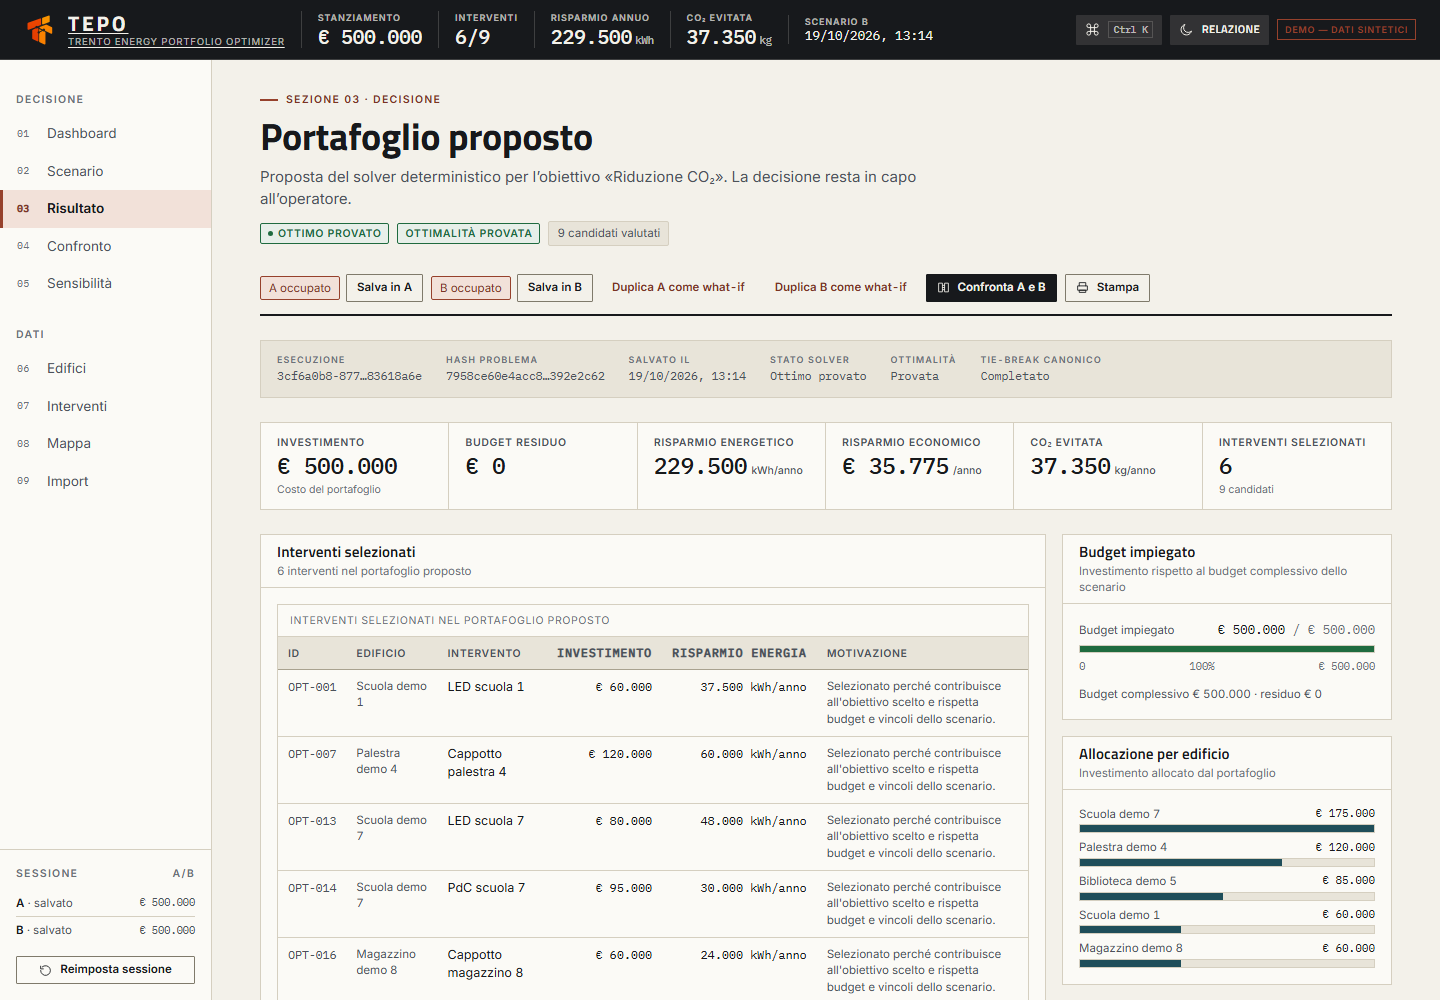
\includegraphics[width=0.95\linewidth]{img/risultato.png}
    \caption{MU-Fig.6 --- Dossier del portafoglio proposto: audit, indicatori, selezionati e allocazione.}
    \label{fig:risultato}
\end{figure}

La Figura~\ref{fig:risultato} mostra il dossier del risultato. In alto sono presenti i comandi per salvare in A o B, duplicare come what-if, confrontare e stampare, insieme ai badge dello stato del solver; segue la fascia di audit con identificativo dell'esecuzione, hash del problema, istante, stato del solver, prova di ottimalità e stato del tie-break. Il dossier riporta poi sei indicatori aggregati, la tabella degli interventi selezionati con la motivazione di ciascuno, l'impiego del budget, l'allocazione dell'investimento per edificio e la sezione ``Perché questa soluzione?'' con il riepilogo delle motivazioni e l'esploratore delle opzioni escluse.

Collegamenti principali: \RFref{rf:risultati}, \RFref{rf:spiegazioni}, \RFref{rf:storico}; UC-07, UC-08, UC-10, UC-11, UC-15; US-07, US-08, US-09, US-11, US-12, US-16.

\subsection{Confronto tra scenari A/B}
\begin{figure}[H]
    \centering
    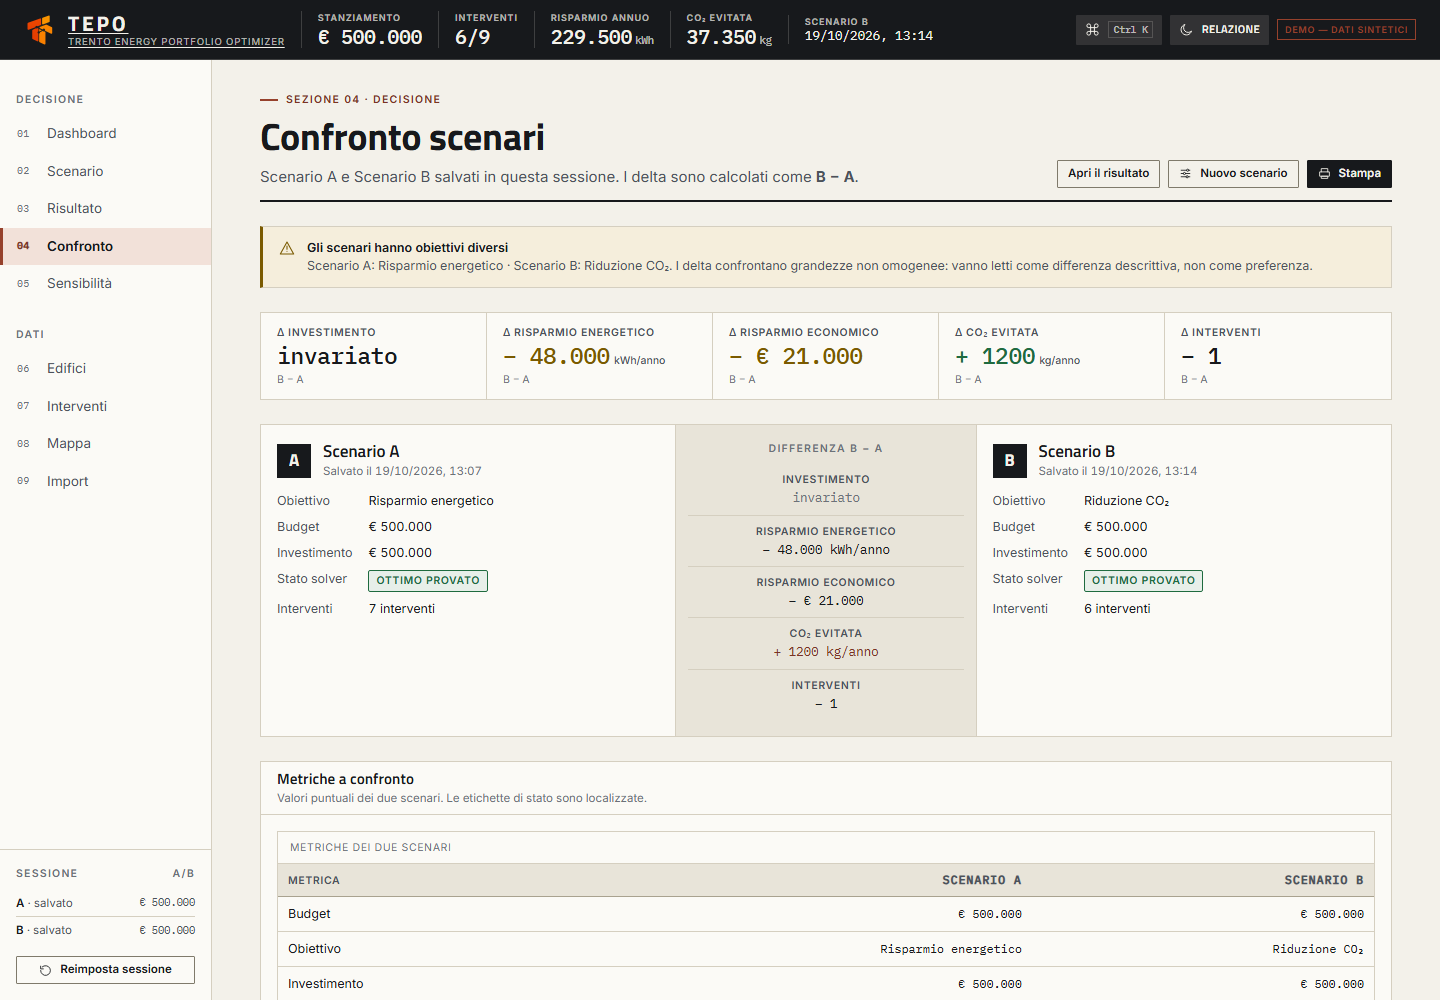
\includegraphics[width=0.95\linewidth]{img/confronto.png}
    \caption{MU-Fig.7 --- Confronto tra Scenario A e Scenario B con delta calcolati come B $-$ A.}
    \label{fig:confronto}
\end{figure}

La Figura~\ref{fig:confronto} mostra il confronto tra due scenari. I due scenari sono affiancati e la colonna centrale riporta gli scostamenti calcolati come $B - A$; in alto sono presenti cinque indicatori di delta (investimento, risparmio energetico, risparmio economico, CO\textsubscript{2} evitata, interventi) e l'eventuale avviso di obiettivi diversi. Seguono la tabella delle metriche a confronto e le sezioni degli interventi aggiunti in B e rimossi rispetto ad A. Sono disponibili i comandi per aprire il risultato, creare un nuovo scenario e stampare.

Collegamenti principali: \RFref{rf:confronto}, \RFref{rf:scenari_salvati}; UC-11, UC-10; US-12, US-11.

\subsection{Mappa degli edifici}
\begin{figure}[H]
    \centering
    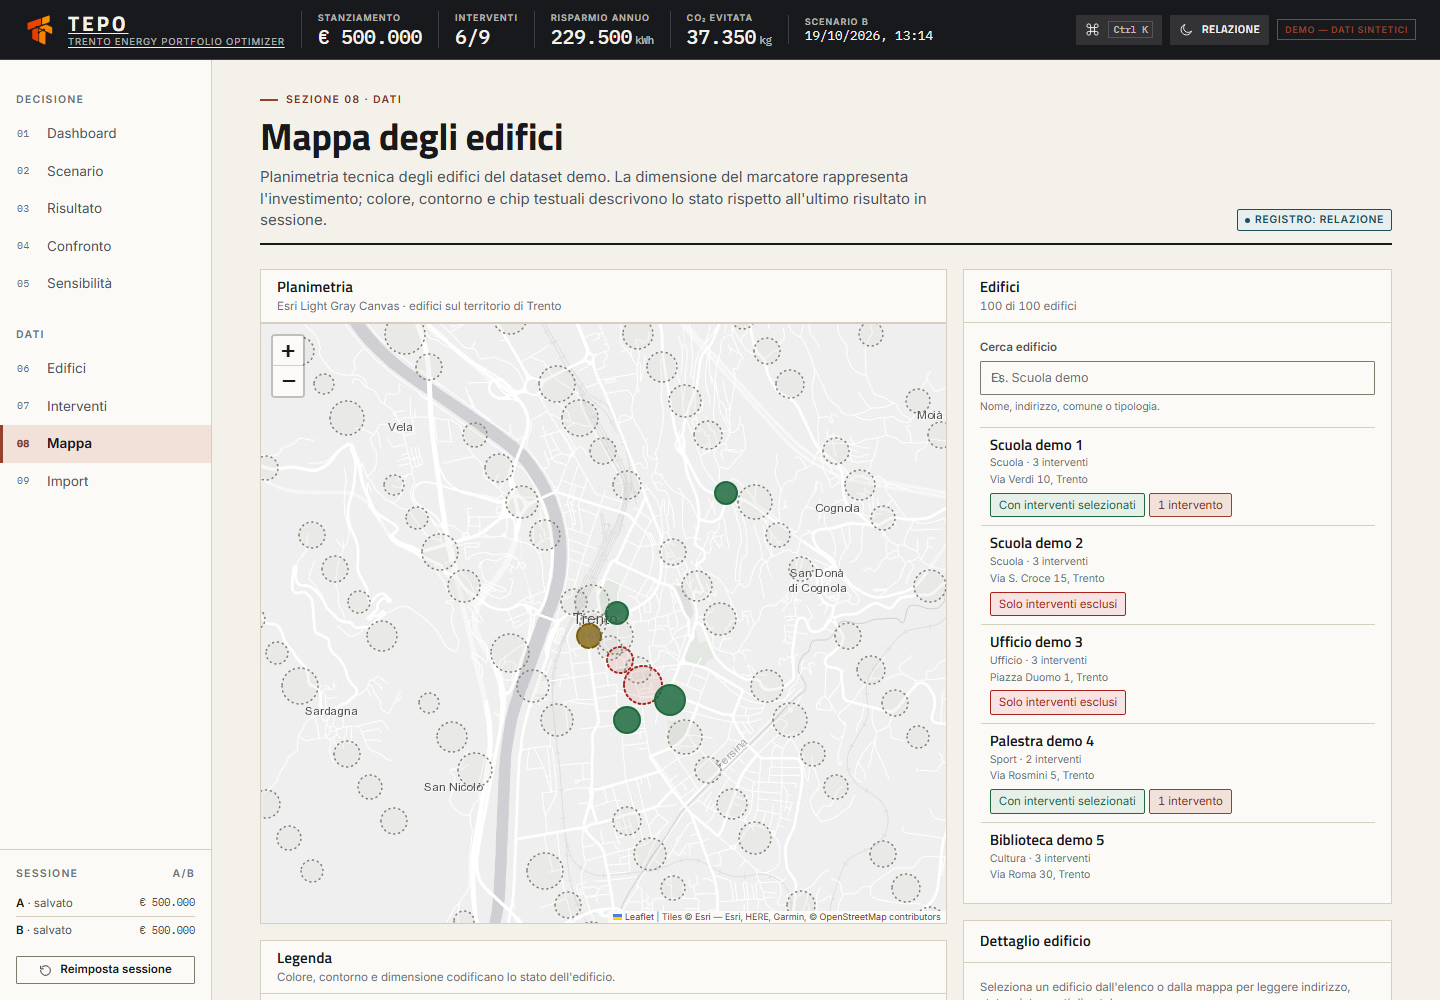
\includegraphics[width=0.95\linewidth]{img/mappa.png}
    \caption{MU-Fig.8 --- Mappa degli edifici con legenda, elenco accessibile e dettaglio dell'edificio.}
    \label{fig:mappa}
\end{figure}

La Figura~\ref{fig:mappa} mostra la mappa degli edifici. La cartografia di base cambia in funzione del registro; i marcatori hanno dimensione proporzionale all'investimento e stato codificato con colore, contorno e etichetta testuale (con interventi selezionati, selezionati ed esclusi, solo esclusi, non valutato). A destra sono presenti la ricerca, l'elenco accessibile degli edifici con lo stato e il pannello di dettaglio dell'edificio selezionato. La legenda e l'attribuzione cartografica sono sempre visibili.

Collegamenti principali: \RFref{rf:mappa}, \RFref{rf:provenienza}; UC-02; US-02, US-17.

\subsection{Analisi di sensibilità sul budget}
\begin{figure}[H]
    \centering
    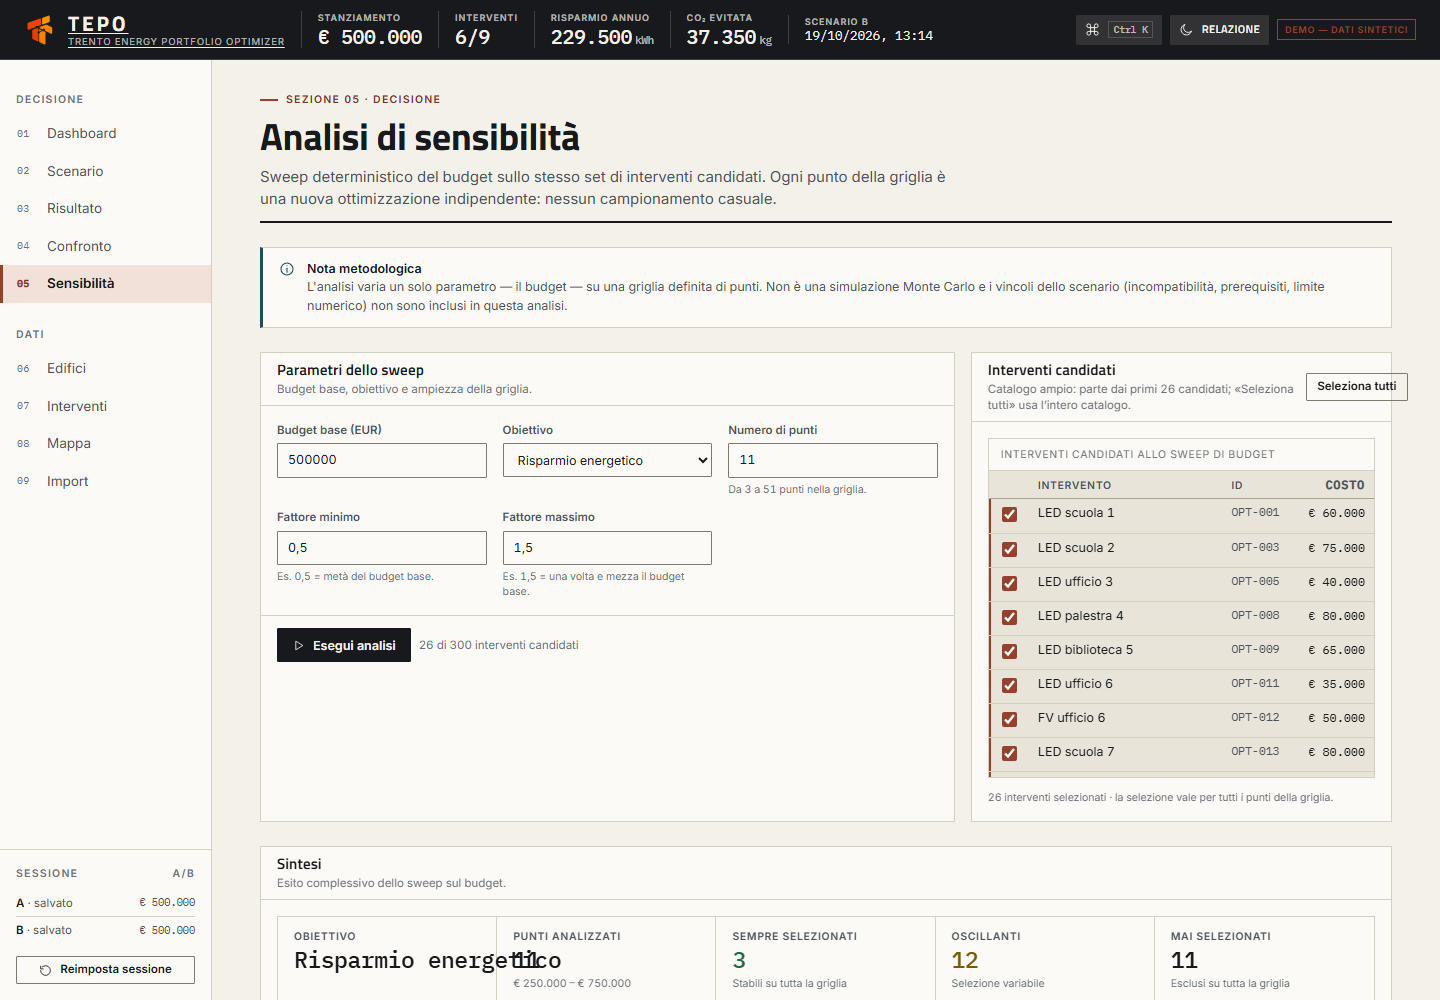
\includegraphics[width=0.95\linewidth]{img/sensibilita.png}
    \caption{MU-Fig.9 --- Analisi di sensibilità: parametri, candidati, nota metodologica e sintesi.}
    \label{fig:sensibilita}
\end{figure}

La Figura~\ref{fig:sensibilita} mostra l'analisi di sensibilità. Sono visibili la nota metodologica (sweep deterministico su un solo parametro, non Monte Carlo, vincoli dello scenario non inclusi), il form con budget base, obiettivo, numero di punti e fattori minimo e massimo, il selettore dei candidati e, in basso, la sintesi con il numero di punti analizzati e la classificazione delle opzioni in sempre selezionate, oscillanti e mai selezionate. Nelle schermate successive della stessa pagina sono presenti il grafico dell'andamento dell'obiettivo, la mappa di selezione per budget e la tabella dei risultati per punto.

Collegamenti principali: \RFref{rf:sensibilita}; UC-12; US-13.

\subsection{Importazione dati da CSV}
\begin{figure}[H]
    \centering
    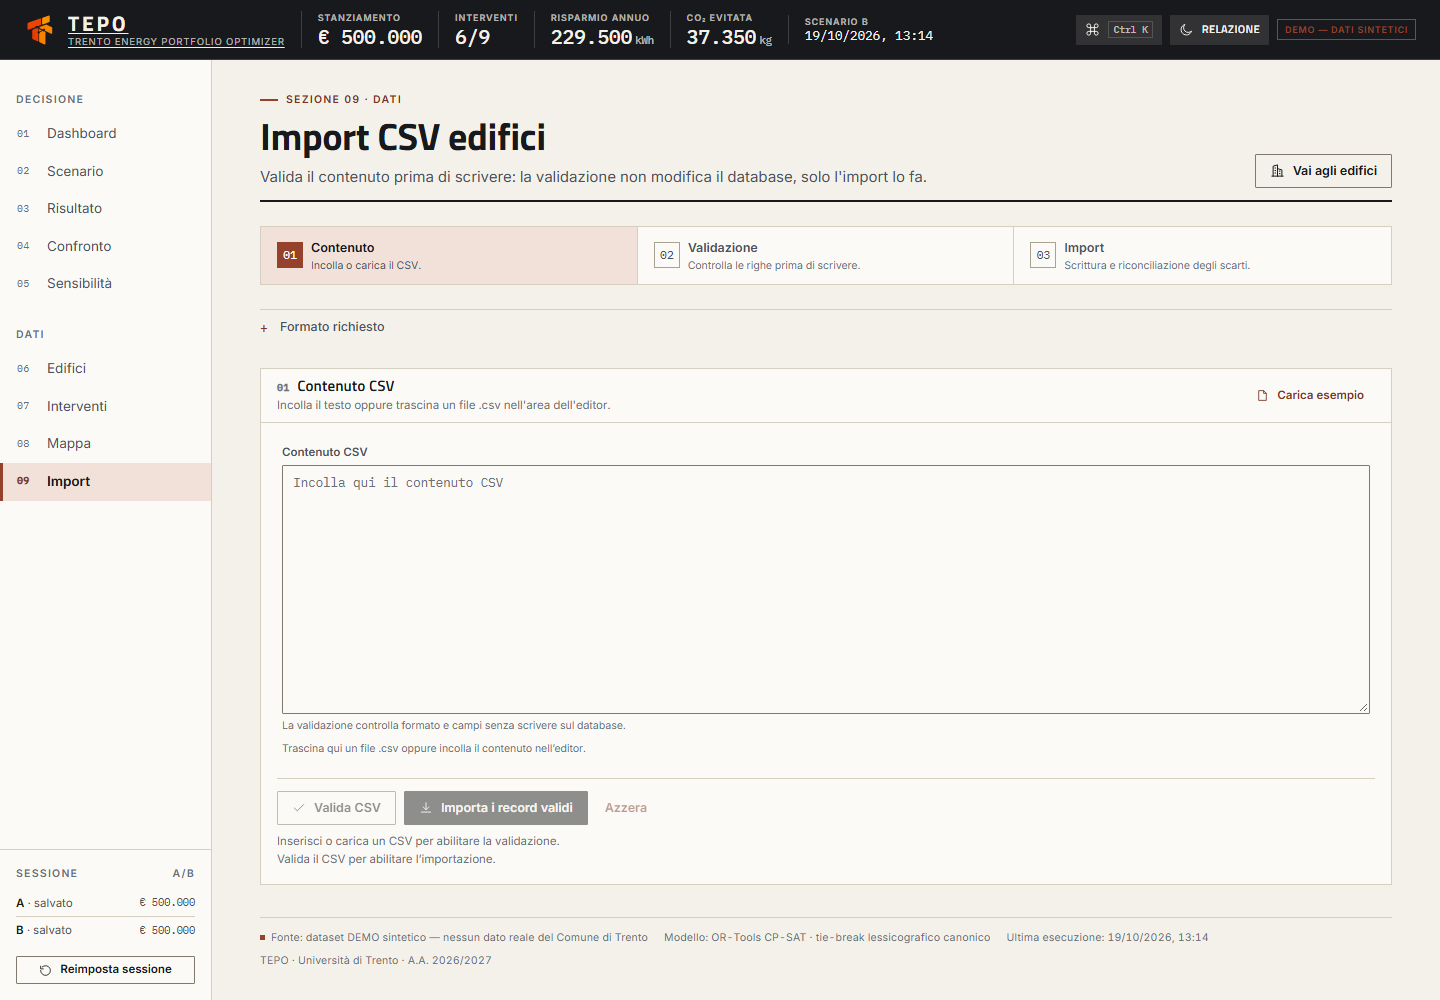
\includegraphics[width=0.95\linewidth]{img/import.png}
    \caption{MU-Fig.10 --- Importazione CSV in tre passi: contenuto, validazione e import.}
    \label{fig:import}
\end{figure}

La Figura~\ref{fig:import} mostra la pagina di importazione, organizzata in tre passi (Contenuto, Validazione, Import). Sono presenti il formato richiesto, l'area per incollare o trascinare il CSV, il comando per caricare un esempio, la validazione a secco, l'anteprima delle righe valide e di quelle scartate con le motivazioni, l'importazione dei soli record validi e la riconciliazione finale degli scarti.

Collegamenti principali: \RFref{rf:import_csv}, \RFref{rf:provenienza}; UC-04; US-04, US-17.

\subsection{Responsività e adattamento}
\begin{figure}[H]
    \centering
    \begin{minipage}[c]{0.30\linewidth}
        \centering
        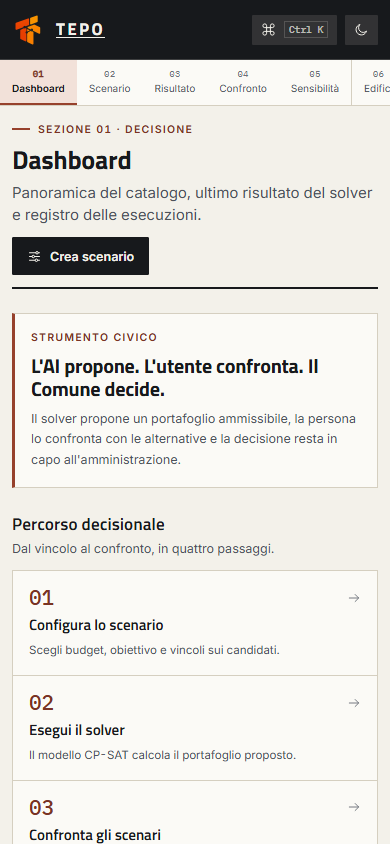
\includegraphics[width=\linewidth]{img/dashboard-mobile.png}
    \end{minipage}\hfill
    \begin{minipage}[c]{0.66\linewidth}
        \centering
        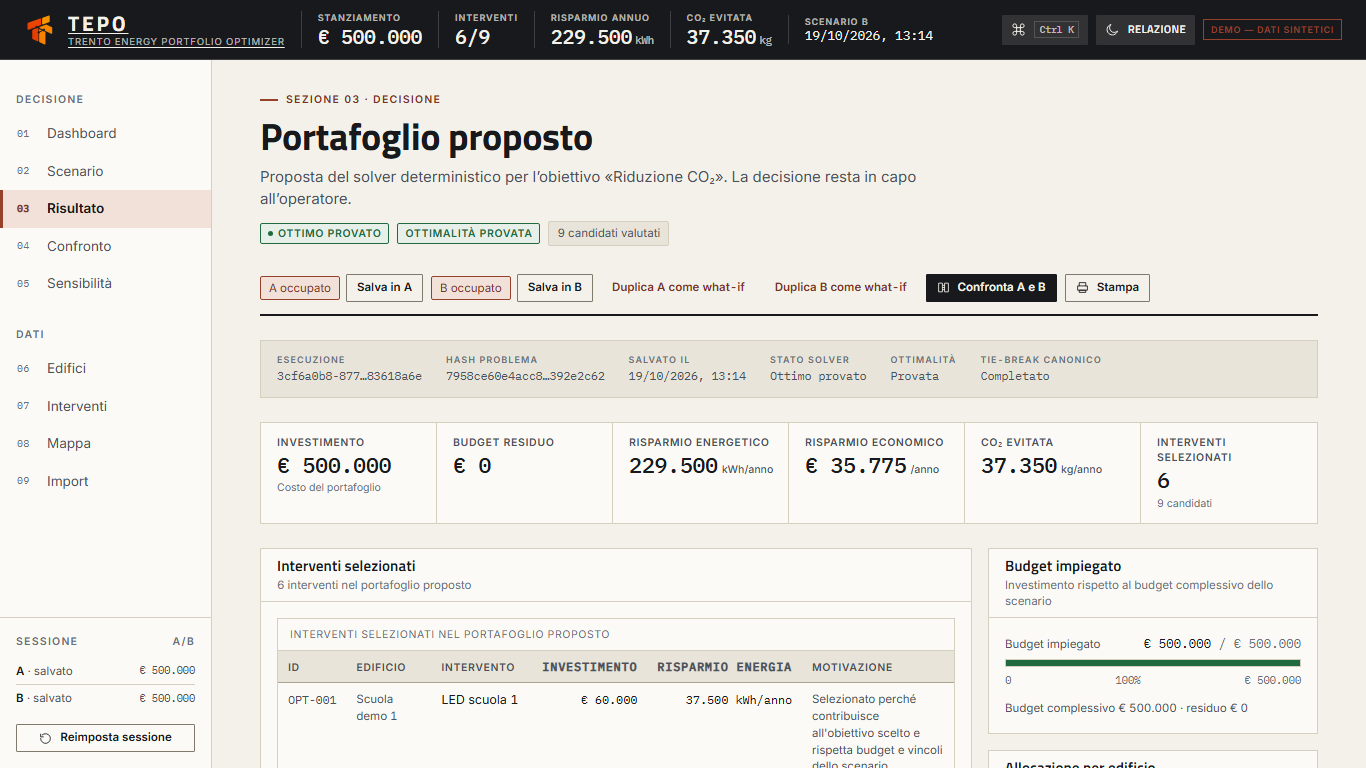
\includegraphics[width=\linewidth]{img/risultato-laptop.png}
    \end{minipage}
    \caption{MU-Fig.11 --- Adattamento del layout: dashboard su viewport mobile (sinistra) e dossier su schermo laptop (destra).}
    \label{fig:responsive}
\end{figure}

La Figura~\ref{fig:responsive} mostra l'adattamento del layout. Su viewport ridotti l'indice laterale diventa una navigazione orizzontale scorrevole, le etichette secondarie della fascia di stato e il timbro demo vengono nascosti, mentre il contenuto resta leggibile; il piè di pagina di provenienza continua a essere disponibile. Su schermi ampi il dossier mantiene la struttura a due colonne con la tabella degli interventi e i pannelli di budget e allocazione. Il layout è progettato per viewport da 320 a 1920 pixel e non comprime le tabelle, che scorrono orizzontalmente quando necessario.

Collegamenti principali: \RFref{rf:risultati}, \RFref{rf:mappa}, \RFref{rf:tema}; \RNFref{rnf:compatibilita}; US-01, US-08, US-16.

\subsection{Nota sugli scostamenti rispetto alla baseline}
Alcune schermate mostrano scelte di prototipo che saranno allineate o motivate nel D2: i vincoli dello scenario demo sono precaricati e mostrati in sola lettura (la modifica puntuale è prevista da \RFref{rf:vincoli_scenario}); l'importazione riguarda attualmente i soli edifici (\RFref{rf:import_csv}); il registro delle esecuzioni nella dashboard mostra un sottoinsieme dei dati di audit, mentre il dettaglio completo è disponibile nel dossier e tramite le API (\RFref{rf:storico}); la scelta del registro è persistita localmente e non è sincronizzata tra dispositivi. Queste differenze non modificano i requisiti della baseline: sono annotate per consentire la verifica nel D2.
